% Template for ICASSP-2019 paper; to be used with:
%          spconf.sty  - ICASSP/ICIP LaTeX style file, and
%          IEEEbib.bst - IEEE bibliography style file.
% --------------------------------------------------------------------------
\documentclass{article}
\usepackage{spconf,amsmath,graphicx}

% Example definitions.
% --------------------
\def\x{{\mathbf x}}
\def\L{{\cal L}}

% Title.
% ------
\title{Using an Attention Mechanism in Discriminative Audio Source Separation}
%
% Single address.
% ---------------
\name{Author(s) Name(s)\thanks{Thanks to XYZ agency for funding.}}
\address{Author Affiliation(s)}
%
% For example:
% ------------
%\address{School\\
%	Department\\
%	Address}
%
% Two addresses (uncomment and modify for two-address case).
% ----------------------------------------------------------
%\twoauthors
%  {A. Author-one, B. Author-two\sthanks{Thanks to XYZ agency for funding.}}
%	{School A-B\\
%	Department A-B\\
%	Address A-B}
%  {C. Author-three, D. Author-four\sthanks{The fourth author performed the work
%	while at ...}}
%	{School C-D\\
%	Department C-D\\
%	Address C-D}
%
\begin{document}
%\ninept
%
\maketitle
%
\begin{abstract}
In this paper, we explore utilizing an attention mechanism in a neural network model for discriminative audio source separation. The attention mechanism enables the model to infer a template vector which best helps to boost the source separation performance. We test our hypothesis on male-female speech mixtures from the TIMIT dataset, and observe that the proposed methodology helps to increase the source-to-distortion ratio on test mixtures. 
\end{abstract}
%
\begin{keywords}
Audio source separation, neural networks, attention mechanism
\end{keywords}
\section{Introduction}
\label{sec:intro}

% little intro on source separation
In audio source separation the goal is to recover the original audio signals in an additive mixture signal. The discriminative source separation models are trained in such a way to directly estimate the underlying sources \cite{ } conditioned on the mixture, as opposed to generative source separation models \cite{ } which first train a generative model separately on the mixtures, which are later to be used for separation \cite{ }. %The current prominent audio source separation methods involve 

% describe attention and model
The attention mechanism was first introduced in the context of automatic machine translation \cite{ }, and then later on used in a variety of computer vision tasks \cite{ } and audio tasks \cite{ }. In this paper, we explore using an attention mechanism in a neural network model to infer \emph{template} vectors in order to enhance the separation performance vectors. In each time instant, the attention mechanism computes a probability vector corresponding to each template. A weighted sum of the chosen templates are then fed into a separator network in addition to the mixture spectrum. 

% talk about the experiment
We perform an extensive search over possible neural network architectures as well as a search over possible hyper-parameter configurations. We test on performing source separation on speech mixtures created using the TIMIT \cite{ } dataset. We observe that the proposed attention mechanism enables a performance boost in terms of source-to-distortion ratio \cite{ }. 

\newcommand{\mix}{x^\text{mix}} 
\newcommand{\ohat}{\hat x^1}
\newcommand{\that}{\hat x^2}
\newcommand{\fohat}{f_{\theta^1}}
\newcommand{\fthat}{f_{\theta^2}}
\newcommand{\srco}{x^1}
\newcommand{\srct}{x^2}

\section{Discriminative Source Separation} 
\label{sec:discsource}

Given a mixture signal $\mix$, the discriminative source separation system $f_\theta = [\fohat, \fthat]$, outputs the estimates $\ohat := \fohat(\mix)$, $\that := \fthat(\mix)$ for the original sources $x^1$ and $x^2$. The system is trained with the following cost function: 
\begin{align}
	\min_\theta \sum_n \left (\|\fohat(\mix_n) - \srco_n \| + \|\fthat(\mix_n) - \srct_n \| \right ), 
\end{align}
where for the sake of simplicity we have omitted the time index to reduce clutter. The neural networks $\fohat$, $\fthat$ can be chosen as multilayer perceptrons, convolutional networks or recurrent neural networks \cite{ }. The diagram of the system is given in Figure \ref{ }. Note that in this paper we are restricting our system to predict two sources, the system described above can be generalized to more than two sources.  

\begin{figure}[h!]
	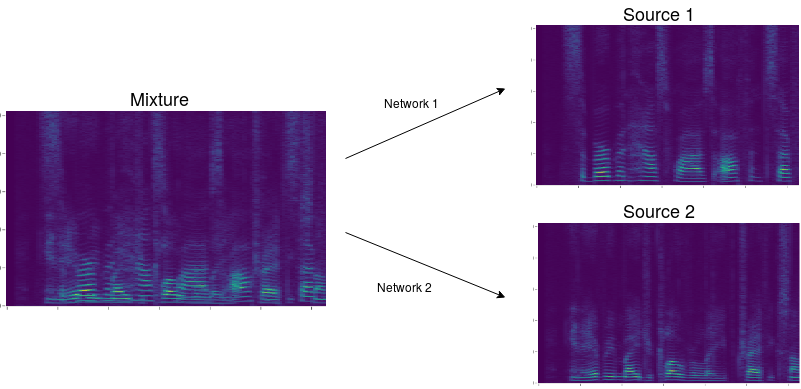
\includegraphics[width=0.45\textwidth]{discsourcesep.png}
	\caption{Discriminative source separation diagram for a two source system} 
\end{figure} 

\section{Attention Mechanism in Discriminative Source Separation} 








% References should be produced using the bibtex program from suitable
% BiBTeX files (here: strings, refs, manuals). The IEEEbib.bst bibliography
% style file from IEEE produces unsorted bibliography list.
% -------------------------------------------------------------------------
\bibliographystyle{IEEEbib}
\bibliography{strings,refs}

\end{document}
